\documentclass[10pt]{beamer}

\usepackage[T1]{fontenc}
\usepackage{amsmath,amssymb,mathtools}
\newcommand{\set}[1]{\left\{ #1 \right \}}

\usepackage{graphicx}
\definecolor{navyblue}{RGB}{0,0,128}
\definecolor{DarkCharcoal}{HTML}{4D4944} 
\colorlet{Charcoal}{DarkCharcoal!85!white} 
\setbeamertemplate{frametitle}
{\begin{centering}\medskip
\bfseries \insertframetitle\par
\end{centering}}

\setbeamertemplate{itemize item}{\textcolor{black}{\textbullet}}
\setbeamercolor{frametitle}{fg=navyblue}
\setbeamercolor{title}{fg=navyblue}

\title{ {\bf Formal Verification of \\
    {\LARGE Neuro-symbolic Multi-agent Systems}}}
\author{ Panagiotis Kouvaros} 
\institute{Verification of Autonomous Systems Group \\Department of Computing, Imperial College London, UK}

\date{August 23, 2023}

\tikzset{
    fig/.style={
        draw=navyblue,
        fill=navyblue,
        rectangle, 
	    inner sep=0.05em
    }
}
    
\newcommand\blfootnote[1]{%
  \begingroup
  \renewcommand\thefootnote{}\footnote{#1}%
  \addtocounter{footnote}{-1}%
  \endgroup
}
\setbeamertemplate{navigation symbols}{
    \insertframenumber/\inserttotalframenumber
}

\begin{document}


%%%%%%%%%%%%%%%%%%%%%%%%%%%%%%%%%%%%%%%%%%%%%%%%%%%%%%%%%%%%%%%%%%%%%%%%%%%%%%

\begin{frame}

    \maketitle


\end{frame}

%%%%%%%%%%%%%%%%%%%%%%%%%%%%%%%%%%%%%%%%%%%%%%%%%%%%%%%%%%%%%%%%%%%%%%%%%%%%%%


\begin{frame}{AI in the Last Decade}

\begin{itemize} \itemsep 2em

    \item Rapid progress  in diverse domains (natural language processing, computer
    vision, autonomous vehicles)

    \item Mainly driven by deep learning (increased computational power, big
        data, improved statistical methods)

    \item Vast potential in revolutionising society

    \item Lack of interpretability and fragility to input perturbations hinders
        adoption in safety-critical applications

    \item Need for verification and neuro-symbolic approaches towards more
        transparent and trustworthy AI

\end{itemize}
 
\end{frame}	

%%%%%%%%%%%%%%%%%%%%%%%%%%%%%%%%%%%%%%%%%%%%%%%%%%%%%%%%%%%%%%%%%%%%%%%%%%%%%%

\begin{frame}{Formal Verification of AI}
	

\begin{itemize}  \itemsep 2em
        \item Formal verification problem
        \begin{large}
		
		\[
            \mathcal S \models \varphi \;\; ?
		\]

		\end{large}

    \item $\mathcal S$ is a multi-agent system comprising {\bf symbolic}, {\bf
        neural} or {\bf neuro-symbolic} agents

    \item $\varphi$ is a specification expressing {\bf temporal-epistemic}, {\bf strategic}
        or {\bf robustness} properties of agents
        
    \end{itemize}

\end{frame}

%%%%%%%%%%%%%%%%%%%%%%%%%%%%%%%%%%%%%%%%%%%%%%%%%%%%%%%%%%%%%%%%%%%%%%%%%%%%%%


\begin{frame}{Verification of Unbounded Multi-agent Systems}


\begin{figure}
\begin{tikzpicture}
\node [fig] (1) {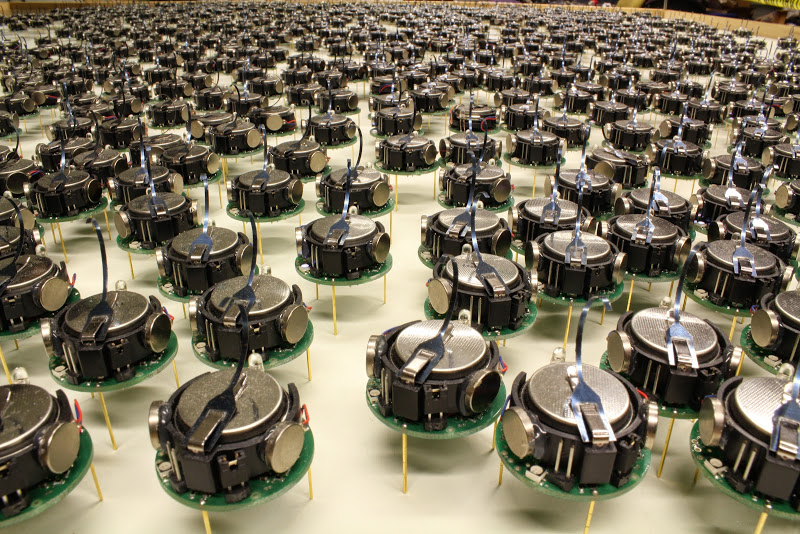
\includegraphics[width=10cm]{images/swarm.jpg}};
\end{tikzpicture}
\end{figure}

\end{frame}

%%%%%%%%%%%%%%%%%%%%%%%%%%%%%%%%%%%%%%%%%%%%%%%%%%%%%%%%%%%%%%%%%%%%%%%%%%%%%%


\begin{frame}{Unbounded Multi-agent Systems}

\begin{itemize} \itemsep 2em
    \item Multi-agent systems composed of an {\bf arbitrary number} of
        homogeneous agents

    \item As in multi-party negotiation protocols and auctions, voting
        protocols, swarm robotics

    \item  Traditional techniques target  verification for
    systems composed of a {\em known} number of agents. 

    \item Need for methods for establishing properties of protocols {\bf
        irrespective of the number of agents} in the system
\end{itemize}

\end{frame}

%%%%%%%%%%%%%%%%%%%%%%%%%%%%%%%%%%%%%%%%%%%%%%%%%%%%%%%%%%%%%%%%%%%%%%%%%%%%%%

\begin{frame}{Parameterised Verification}

    \begin{itemize} \itemsep 1em 

        \item {\bf Parameterised Interleaved Interpreted Systems}: a {\em
    parameterised} semantical structure, where the parameter is the number of
    agents in the system

    \item {\bf IACTLK}: an \emph{indexed} version of the
        temporal-epistemic logic  ACTLK that allows for quantifying over 
        the agents
        \begin{itemize}
            \item[\textcolor{black}{-}] {\em Connectedness} property:
                $\forall i \colon AGAF\sf{connected}(i)$
            (``every robot is infinitely often close to another robot'')
        \end{itemize}
    %expressing properties irrespective of the number of agents in the
	%system.

\item {\bf Parameterised model checking problem:}

	Input: A PIIS  $\mathcal{S}$  and an IACTLK formula $\varphi$

	Output:
	\begin{itemize}
        \item[\textcolor{black}{-}] {\em Yes} if $\forall n \in \mathbb{N} \;\; \colon \;\;
			\mathcal{S}(n) \models
	 \varphi$.
        \item[\textcolor{black}{-}] {\em No} otherwise
	\end{itemize}

\item The parameterised model checking problem for PIIS  is in general {\bf
    undecidable}
            %~\footnote{P. Kouvaros, A. Lomuscio. {\em Parameterised
            %Verification for Multi-agent Systems.} Artificial Intelligence}
    \end{itemize} 

\end{frame}

%%%%%%%%%%%%%%%%%%%%%%%%%%%%%%%%%%%%%%%%%%%%%%%%%%%%%%%%%%%%%%%%%%%%%%%%%%%%%%

\begin{frame}{Cutoffs} 
 
\begin{itemize} \itemsep 2em
    \item A natural number   $c \in \mathbb{N}$ is said to be
        a {\bf cutoff} for a PIIS $\mathcal{S}$ and a formula $\varphi$ if
  \[ 
        \forall n \in [1, c]  \; \colon \; \mathcal{S}(c) \models \varphi \;\;
   \Leftrightarrow \;\; \forall n \geq 1 \; \colon  \;
    \mathcal{S}(n) \models \varphi
 \]

\item  If a cutoff exists, then the PMCP can be solved by checking  all
    the concrete systems up to the cutoff


\item  The existence and computability of cutoffs depends on the
    synchronisation primitives endowing the agents
\end{itemize}


\end{frame}

%%%%%%%%%%%%%%%%%%%%%%%%%%%%%%%%%%%%%%%%%%%%%%%%%%%%%%%%%%%%%%%%%%%%%%%%%%%%%%


\begin{frame}{Synchronisations and Cutoffs in PIIS}
 
\begin{itemize}  \itemsep 2em

        \item {\bf Fully synchronous} semantics always admit cutoffs (identification procedure in exponential time)


    \item {\bf Asynchronous} semantics with {\bf broadcast} communication
        primitives always admit cutoffs (identification procedure in linear time)
        
    \item {\bf Asynchronous} semantics with {\bf broadcast} and {\bf
        agent-environment} communication primitives admit cutoffs under the
        condition  that the environment can never block pairwise
        synchronisations for the system of one agent only (identification
        procedure in exponential time)

    
    \item Same condition holds for {\bf multi-role systems} with 
        pairwise communication between agents of different roles

\end{itemize}


\end{frame}

%%%%%%%%%%%%%%%%%%%%%%%%%%%%%%%%%%%%%%%%%%%%%%%%%%%%%%%%%%%%%%%%%%%%%%%%%%%%%%

\begin{frame}{Fault-tolerance}

\begin{itemize} \itemsep 2em
        \item Adverse functioning behaviour of some of the agents in the system 
        \begin{itemize}
            \item[\textcolor{black}{-}]Could a faulty robot break a flying formation?
        \end{itemize}
        \item Combined with fault-injection  techniques parameterised verification
    can be used to establish the robustness of a UMAS to faults

        \item Additionally, adaptations of the labelling algorithm for CTLK can
            be used to  compute the {\bf maximum ratio of faulty to non-faulty
            agents} that the system can tolerate with respect to a specification
\end{itemize}

\end{frame}

%%%%%%%%%%%%%%%%%%%%%%%%%%%%%%%%%%%%%%%%%%%%%%%%%%%%%%%%%%%%%%%%%%%%%%%%%%%%%%

\begin{frame}{MCMAS-P}

\begin{itemize}
    \item Traditional verification can verify the Alpha swarm aggregation
        algorithm only up to 7 robots, whereas \texttt{MCMMAS-P} establishes
        the correctness of the protocol for any number of agents.
\end{itemize}
\vspace{1em}

\begin{tikzpicture}
\node [fig, fill=white, line width = 0.025cm] (1) {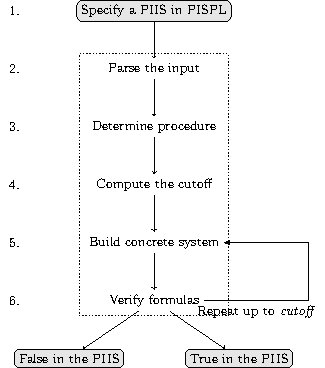
\includegraphics[width=5cm]{images/mcmasp.pdf}};
\node [fig, fill=white, line width = 0.025cm, yshift=3em,xshift=15em] (1) {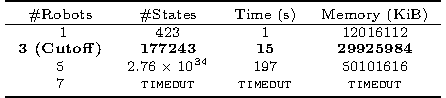
\includegraphics[width=7.5cm]{images/exp.pdf}};
\end{tikzpicture}

\end{frame}

%%%%%%%%%%%%%%%%%%%%%%%%%%%%%%%%%%%%%%%%%%%%%%%%%%%%%%%%%%%%%%%%%%%%%%%%%%%%%%

\begin{frame}{Verification of Neural Networks}

    \begin{figure}
        \begin{tikzpicture}
        \node [fig, fill=white, line width = 0.025cm] (1) {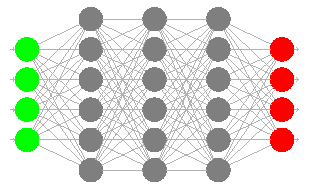
\includegraphics[width=5cm]{images/neuralagent.pdf}};
        \node [fig, fill=white, line width = 0.025cm, xshift=13.5em] (1) {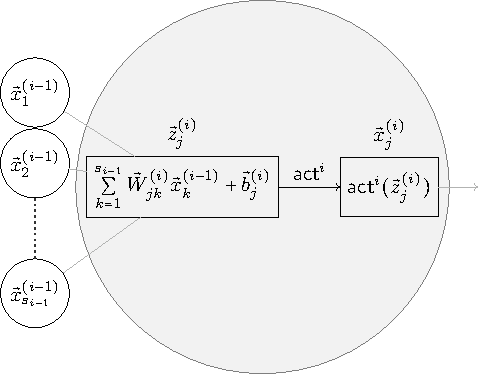
\includegraphics[width=4cm]{images/node.pdf}};
        \end{tikzpicture}
        \end{figure}


\end{frame}

%%%%%%%%%%%%%%%%%%%%%%%%%%%%%%%%%%%%%%%%%%%%%%%%%%%%%%%%%%%%%%%%%%%%%%%%%%%%%%

\begin{frame}{Fragility of Neural Networks}

\begin{itemize}
    \item Imperceptible perturbations to the inputs often cause networks to
        miss-classify

        \vspace{2em}

    \begin{figure}
        \begin{tikzpicture}
        \node [fig, fill=white, line width = 0.025cm] (1) {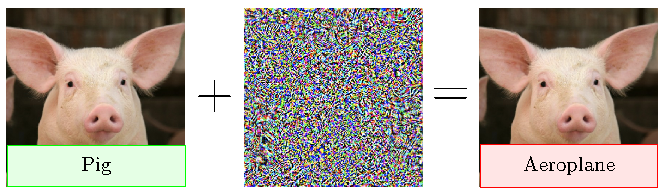
\includegraphics[width=10cm]{images/advrob.pdf}};
        \end{tikzpicture}
        \end{figure}
\end{itemize}

\end{frame}

%%%%%%%%%%%%%%%%%%%%%%%%%%%%%%%%%%%%%%%%%%%%%%%%%%%%%%%%%%%%%%%%%%%%%%%%%%%%%%

\begin{frame}{Formal Verification Problem}
\begin{itemize} \itemsep 1.5em
    \item Aims to establish whether neural networks behave as intended in
        regions of the input space:
        \[
            \forall \vec x \in \mathcal X \colon \vec f(\vec x) \in \mathcal Y,
        \]
        where $\vec f$ is a network, $\mathcal X$  is a set of inputs and
        $\mathcal Y$ is a set of outputs of the network
    
    \item {\bf Reachability} and {\bf local robustness} properties are instantiated from 
        from above

    \item Robustness against certain input perturbations denoting $\mathcal
        X$ is particularly important in assuring safe behaviour in the
        operation domain
\end{itemize}

\end{frame}

%%%%%%%%%%%%%%%%%%%%%%%%%%%%%%%%%%%%%%%%%%%%%%%%%%%%%%%%%%%%%%%%%%%%%%%%%%%%%%

%\begin{frame}{Formal Verification Problem}

%%\documentclass{standalone}

%\usepackage[T1]{fontenc}
\usepackage{amsmath,amssymb,mathtools}
\newcommand{\set}[1]{\left\{ #1 \right \}}

%\usepackage{graphicx}
%\definecolor{navyblue}{RGB}{0,0,128}

%\begin{document}

	\begin{tikzpicture}[node distance=1.45cm,  minimum
	  height=0.7cm,font=\scriptsize] 

        \node[] (l0) {{\scriptsize {\bf Input}}};
	\node[right of =l0, xshift=11.25em] (1) {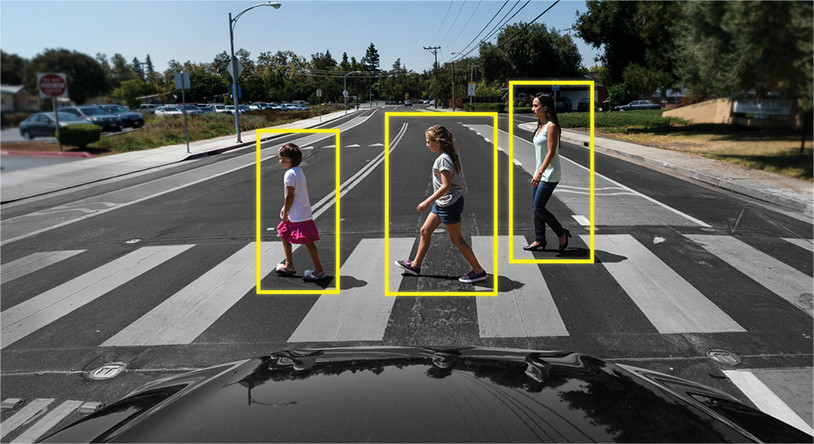
\includegraphics[width=1.4cm]{images/pedestrian.jpg}};
    \node[below of=1, yshift=2.25em] (x1) {{\large $\downarrow$}};

        \node[below of = l0] (l1) {{\scriptsize{\bf Perturbations}}};
        \node[label={[below, yshift=-2em]{\scriptsize Brightness}}, right of=l1,below of =l0, xshift=1em] (2) {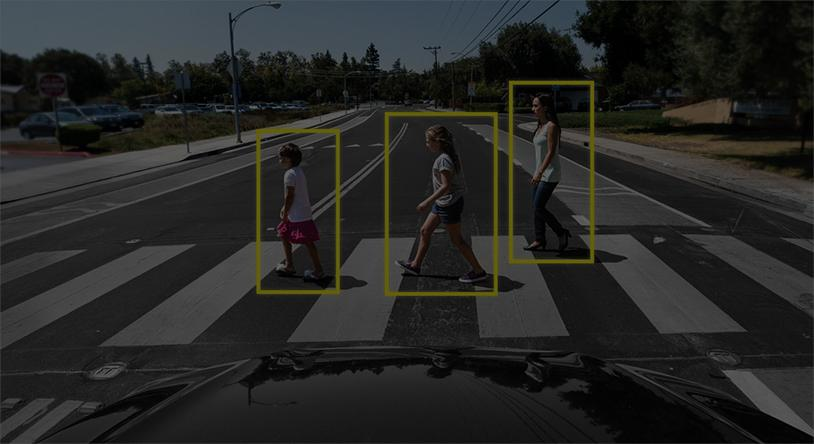
\includegraphics[width=1.4cm]{images/pedestrian_brightness.jpg}};
        \node[label={[below, yshift=-2em]{\scriptsize Contrast}}, right of =2] (3) {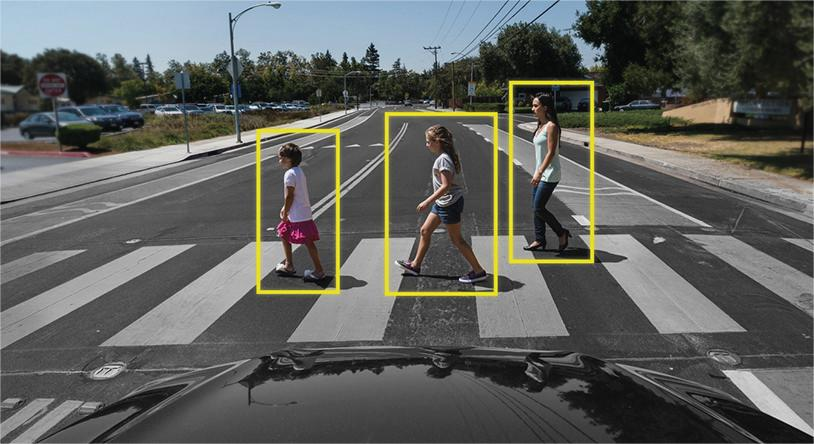
\includegraphics[width=1.4cm]{images/pedestrian_contrast.jpg}};
        \node[label={[below, yshift=-2em] {\scriptsize White noise}}, right of =3] (4) {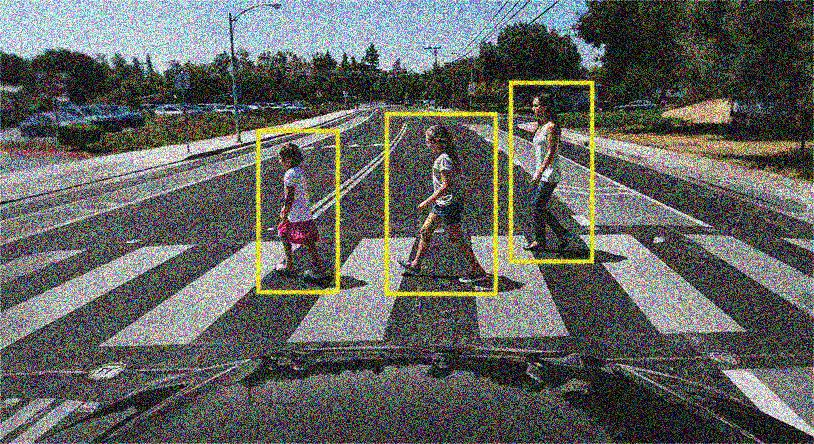
\includegraphics[width=1.4cm]{images/pedestrian_noise.jpg}};  
        \node[label={[below, yshift=-2em] {\scriptsize Rotate}}, right of =4] (5) {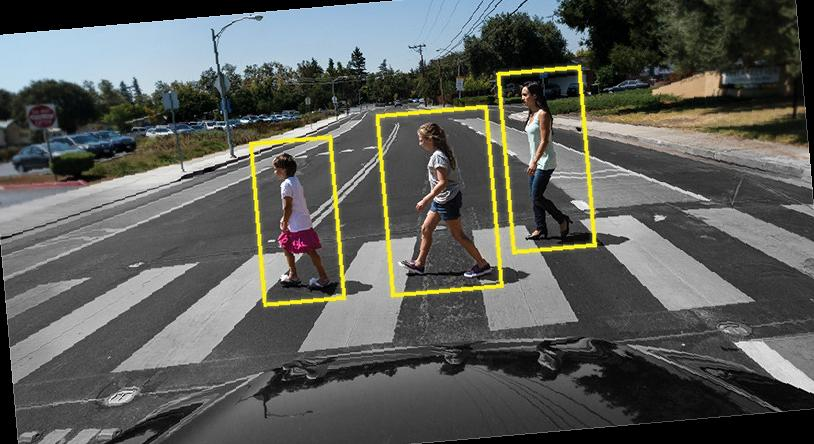
\includegraphics[width=1.4cm]{images/pedestrian_rotate.jpg}};
        \node[label={[below, yshift=-2em] {\scriptsize Scale}}, right of =5] (6) {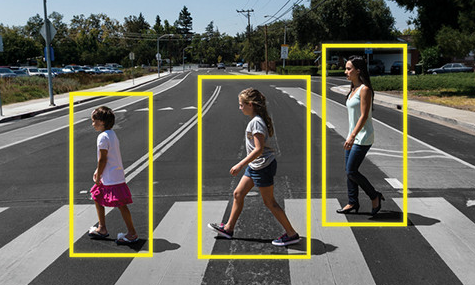
\includegraphics[width=1.3cm]{images/pedestrian_scale.png}};
        \node[label={[below, yshift=-2em] {\scriptsize Hue}}, right of =6] (7) {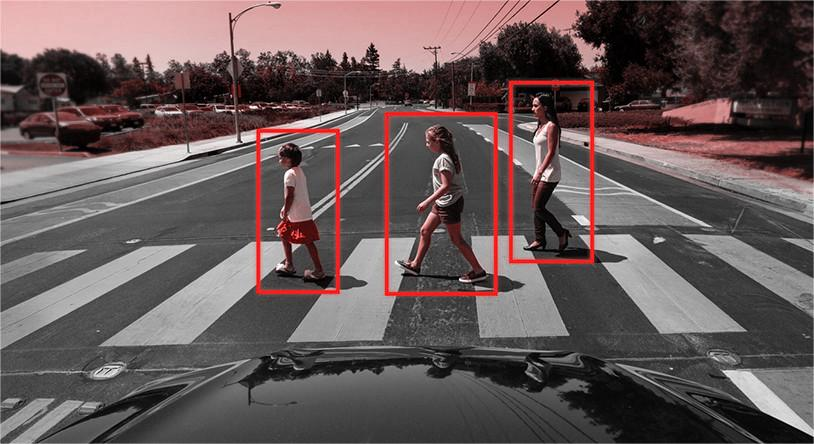
\includegraphics[width=1.4cm]{images/pedestrian_hue.jpg}};



        \node[below of = l1] (l2) {{\scriptsize{\bf Verification}}};

        \node[below of = x1, yshift=-1em] (x2) {{\large $\downarrow$}};
        \node[fig, fill=white, minimum width=3cm,rectangle, rounded corners, below of=x2, yshift=2.3em] (v) {{\bf Verification tool}};
        \node[left  of = v, xshift=-1.25em] (x4) {{\large $\rightarrow$}};
        \node[left of = x4, xshift=1.25em] (x3) {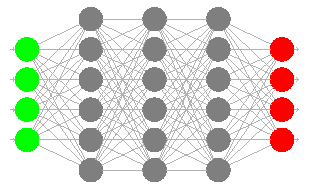
\includegraphics[width=0.15\textwidth]{images/neuralagent.pdf}};

        \node[below of = v, yshift=2em] (x2) {{\large $\downarrow$}};
        \node[below of = l2, yshift=-2em, align=center] (l3) {{\scriptsize{\bf Certification /}} \\ {\scriptsize {\bf Fragilities}}};

        \node[rectangle, fill=green!30, below of =2, yshift=-5em] {Robust};
        \node[rectangle, fill=red!30, below of =3, yshift=-5em] (y1) {Not robust};
        \node[below of = y1, yshift=1.9em] (x3) {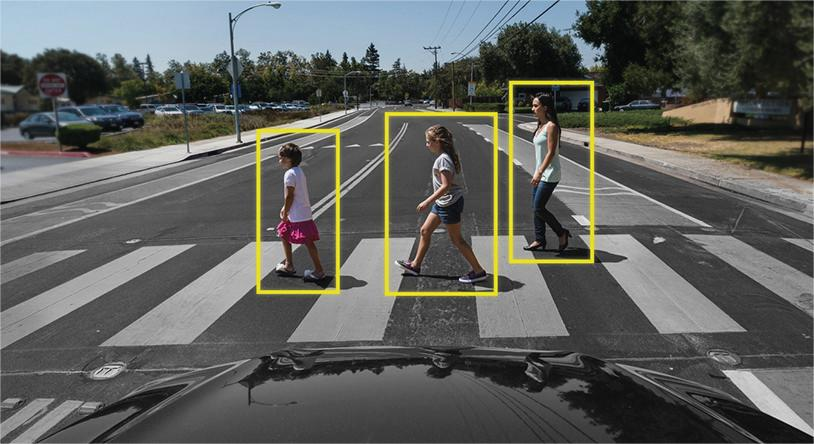
\includegraphics[width=0.13\textwidth]{images/pedestrian_contrast.jpg}};
        \node[rectangle, fill=green!30, below of =4, yshift=-5em] {Robust};
        \node[rectangle, fill=green!30, below of =5, yshift=-5em] {Robust};
        \node[rectangle, fill=red!30, below of =6, yshift=-5em] (y2) {Not robust};
        \node[below of = y2, yshift=1.9em] (x3) {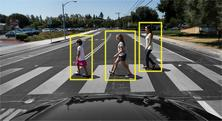
\includegraphics[width=0.13\textwidth]{images/pedestrian_scale.jpg}};
        \node[rectangle, fill=green!30, below of =7, yshift=-5em]{Robust};

        
  \path[-latex,semithick,every node/.style={->,font=\sffamily\normalsize, scale=0.9}]
        (l0) edge (l1)
        (l1) edge (l2)
        (l2) edge (l3);
        
        \node[fit=(1)(2)(7)(x3), draw=navyblue, line width=0.025cm, inner sep=0em] {};

  \end{tikzpicture}
%\end{document}


%\end{frame}



%%%%%%%%%%%%%%%%%%%%%%%%%%%%%%%%%%%%%%%%%%%%%%%%%%%%%%%%%%%%%%%%%%%%%%%%%%%%%%


%\begin{frame}{Verification methods}

%\begin{itemize} \itemsep 2em
    
%\item {\bf Complete methods}
    %\begin{itemize}    
        %\item[\textcolor{black}{-}] exact representations of the verification problem
        %\item[\textcolor{black}{-}]always answer the verification problem (given enough
            %time)
        %\item[\textcolor{black}{-}] low scalability
        %\item[\textcolor{black}{-}] work focuses on improving scalability
    %\end{itemize}	

%\item {\bf Incomplete methods} 
    %\begin{itemize}
        %\item[\textcolor{black}{-}] relaxations of the verification problem
        %\item[\textcolor{black}{-}]high scalability
        %\item[\textcolor{black}{-}] answer the verification problem only some of the time
        %\item[\textcolor{black}{-}] work focuses on improving precision
    %\end{itemize}	

%\end{itemize}
%\vspace{1em}
	

%\blfootnote{{\bf P. Kouvaros}, A. Lomsucio. {\em Towards Scalable Complete Verification of ReLU Neural Networks via Dependency-based Branching}. IJCAI21}
%\blfootnote{V. Hasemi, {\bf P. Kouvaros}, A. Lomsucio. {\em OSIP: Tightened
    %Bound Propagation for the Verification of ReLU Neural Networks}. SEFM21}
%\blfootnote{B. Batten, {\bf P. Kouvaros}, A. Lomsucio, Y. Zheng. {\em Efficient Neural Network Verification via Layer-based Semidefinite Relaxations and Linear Cuts}. IJCAI21}
%\blfootnote{E. Botoeva, {\bf P. Kouvaros}, J. Kronqvist, R. Misener. {\em Efficient Verification of ReLU-based Neural Networks via Dependency Analyis.} AAAI20}

%Various work on incomplete verification towards improving precision [IJCAI21,
    %SEFM21] and compete verification towards improving scalability [AAAI20,
    %IJCAI21].

%\vspace{1em}

%In this talk I will focus on complete verification.


%\end{frame}

%%%%%%%%%%%%%%%%%%%%%%%%%%%%%%%%%%%%%%%%%%%%%%%%%%%%%%%%%%%

%%%%%%%%%%%%%%%%%%%%%%%%%%%%%%%%%%%%%%%%%%%%%%%%%%%%%%%%%%%%%%%%%%%%%%%%%%%%%%


\begin{frame}{ReLU Networks}


\begin{columns}

	\begin{column}{0.45\textwidth}
	\begin{large}
	\[
	y(x) = \max(0,x)
	\]
	\end{large}

	\begin{itemize}
        \item ReLU is {\bf piecewise-linear}
        \item When $x \geq 0$ the node is said to be in the { \bf active
			state}
			and outputs $x$

        \item When $x < 0$ the node is said to be in the {\bf inactive state}
			and outputs $0$
	\end{itemize}
\end{column}
\begin{column}{0.5\textwidth}

    \begin{figure}
        \begin{tikzpicture}
        \node [fig, fill=white, line width = 0.025cm] (1) {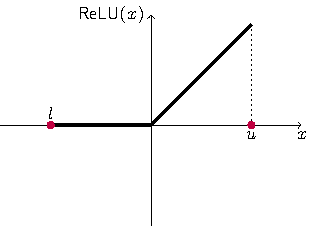
\includegraphics[width=5cm]{images/relaxation.pdf}};
        \end{tikzpicture}
        \end{figure}

\end{column}
\end{columns}

\end{frame}

%%%%%%%%%%%%%%%%%%%%%%%%%%%%%%%%%%%%%%%%%%%%%%%%%%%%%%%%%%%%%%%%%%%%%%%%%%%%%%

\begin{frame}{MILP Compilation}

\begin{itemize} \itemsep 1em
    \item The verification problem is recast into a MILP program
        \vspace{1em}
        \begin{figure}
        \begin{tikzpicture}
        \node [fig] (1) {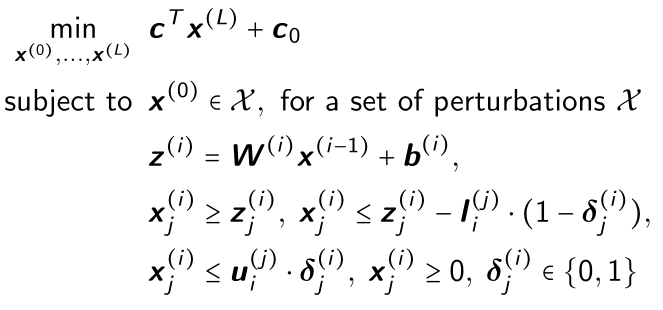
\includegraphics[width=6cm]{images/relu_milp.png}};
        \end{tikzpicture}
        \end{figure}

    \item The verification problem is satisfied iff its MILP encoding has no
feasible solution

    \item Any feasible solution corresponds to an input violating the robustness of the network

    \item Perfomance greatly depends on the tightness of the pre-activation
        bounds and the  number of binary variables encoding the ReLU non-linerarities
\end{itemize}

\end{frame}

%%%%%%%%%%%%%%%%%%%%%%%%%%%%%%%%%%%%%%%%%%%%%%%%%%%%%%%%%%%%%%%%%%%%%%%%%%%%%%

\begin{frame}{Improved Scalability}

\begin{itemize} \itemsep 2em


\item {\bf Symbolic interval propagation} enables fast, gpu-accelerated
    symbolic derivation of tights bounds through linear relaxations of the ReLU
        nodes
    \vspace{1em}
    \begin{itemize} 
    \item[\textcolor{black}{-}] The bounds can be further tightned by acounting
        for intra-layer dependencies, instead of simply relying on local over-
        approximation areas, when choosing a relaxation
\end{itemize}


\item {\bf Dependency analysis} exploits relations whereby the  operational
    states of the ReLUs for a set of inputs is connected by logical implication
    \vspace{1em}
    \begin{itemize} \itemsep 1em
        \item[\textcolor{black}{-}] Using MILP cuts
        \item[\textcolor{black}{-}] Using branching heuristics
    \end{itemize}
\end{itemize}
\end{frame}

%%%%%%%%%%%%%%%%%%%%%%%%%%%%%%%%%%%%%%%%%%%%%%%%%%%%%%%%%%%%%%%%%%%%%%%%%%%%%%

%\begin{subequations} 
%\begin{align*}
    %\min_{\activation 0, \ldots, \activation L} \;\; & \vec c^T
    %\activation L + \vec c_0
    %\nonumber \\
    %\text{subject to} \;\;   &  \activation 0 \in \mathcal{X}, 
    %\text{ for a set of perturbations } \mathcal X 
    %\nonumber \\
    %& \preact i = \weights i \activation{i-1} + \bias i,  \nonumber \\
    %& \activation i_j \geq  \preact i_j,  \; 
     %\activation i_j \leq \preact i_j - \outlb{i}^{(j)} \cdot (1 -
    %\deltavar{i}{j}), \nonumber \nonumber \\
    %& \activation i_j \leq \outub{i}^{(j)} \cdot \deltavar{i}{j}, \;
    %\activation i_j \geq 0, \;
    %\deltavar{i}{j} \in \set{0,1} \nonumber \\
%\end{align*}
%\end{subequations}

%\begin{block}{MILP compilation of node~$q$ in layer~$i$}
%\begin{align*}
%&\out{i,q} \geq 0 \\
%&\out{i,q} \geq \pre{i,q} \\
%&\out{i,q} \leq \preub{i,q} \cdot \delta_{i,q} \\
%&\out{i,q} \leq \pre{i,q} - \prelb{i,q} \cdot (1 - \delta_{i,q})
%\end{align*}
%where $\out{i,q}$ is the output of the node, $\pre{i,q}$ its
%pre-activation, $\prelb{i,q}$ a lower bound of the pre-activation,
%$\preub{i,q}$ an upper bound of the pre-activation and $\delta_{i,q}$ a
%binary variable.
%\end{block}


%%%%%%%%%%%%%%%%%%%%%%%%%%%%%%%%%%%%%%%%%%%%%%%%%%%%%%%%%%%%%%%%%%%%%%%%%%%%%%

%\begin{frame}{Bound derivation}

%\begin{itemize}

    %\item {\bf Symbolic interval propagation} enables the symbolic derivation of the bounds using linear relaxations of the ReLU nodes

%\item Improved precision via {\bf joint optimisations} of the relaxations 

%\begin{figure}
%\begin{tikzpicture}
%\node [fig, fill=white, line width=0.025cm] (1) {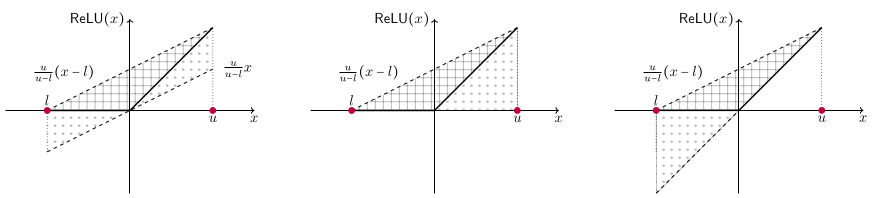
\includegraphics[width=8cm]{images/relaxations.png}};
%\end{tikzpicture}
%\end{figure}

%\item Even tighter (albeit slower) methods use {\bf semidefinite programming} relaxations 

%\begin{figure}
%\begin{tikzpicture}
%\node [fig, fill=white, line width=0.025cm] (1) {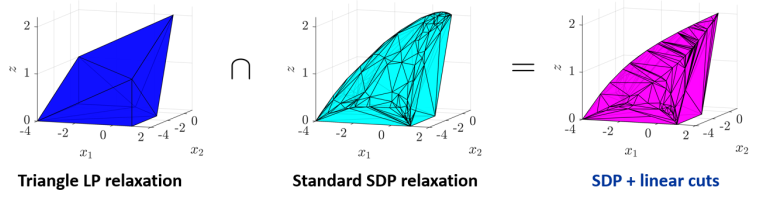
\includegraphics[width=8cm]{images/sdp.png}};
%\end{tikzpicture}
%\end{figure}

%\end{itemize} 

%\blfootnote{B. Batten, {\bf P. Kouvaros}, A. Lomsucio, Y. Zheng. {\em Efficient Neural Network Verification via Layer-based Semidefinite Relaxations and Linear Cuts}. IJCAI21}
%\blfootnote{V. Hasemi, {\bf P. Kouvaros}, A. Lomsucio. {\em OSIP: Tightened
    %Bound Propagation for the Verification of ReLU Neural Networks}. SEFM21}

%\end{frame}



%%%%%%%%%%%%%%%%%%%%%%%%%%%%%%%%%%%%%%%%%%%%%%%%%%%%%%%%%%%%%%%%%%%%%%%%%%%%%%

%\begin{frame}{Branch-and-bound}
%\begin{itemize} \itemsep 1.5em
%\item Relax all integrality constraints to linear ones
%\item Solve the resulting linear program
%\item If all integrality constraints are satisfied then terminate
%\item Otherwise, branch on an integral variable and repeat for each
    %resulting sub-problem
%\end{itemize}
%\vspace{1em}

%\begin{figure}
%\begin{tikzpicture}
%\node [fig, fill=white, line width=0.025cm] (1) {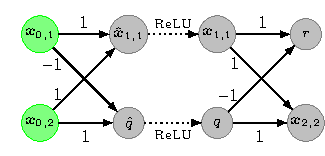
\includegraphics[width=4.5cm]{images/net_no_bounds.pdf}};
%\node [fig, fill=white, right of=1, xshift=8.25em, line width=0.025cm] (1) {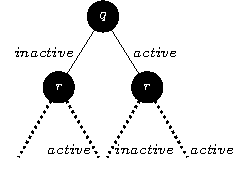
\includegraphics[width=3cm]{images/tree_no_cross.pdf}};
%\end{tikzpicture}
%\end{figure}

%\end{frame}



%%%%%%%%%%%%%%%%%%%%%%%%%%%%%%%%%%%%%%%%%%%%%%%%%%%%%%%%%%%%%%%%%%%%%%%%%%%%%%

%\begin{frame}{Dependencies}
%\begin{itemize} \itemsep 2em
    %\item {\bf Key limitation} of branch-and-bound: the resulting search space
        %is exponential in the number of ReLU nodes in the network

    %\item  {\bf Dependency analysis} aims at reducing the search space during
        %branch-and-bound

    %\item  An unstable (i.e., neither active nor inactive) node $r$ is said to
        %{\bf depend} on an unstable node $q$ if whenever $q$ is stable, $r$ is stable
        %as well
            
%\end{itemize}

%\blfootnote{E. Botoeva, {\bf P. Kouvaros}, J. Kronqvist, R. Misener. {\em Efficient Verification of ReLU-based Neural Networks via Dependency Analyis.} AAAI20}
%\end{frame}

%%%%%%%%%%%%%%%%%%%%%%%%%%%%%%%%%%%%%%%%%%%%%%%%%%%%%%%%%%%%%%%%%%%%%%%%%%%%%%

%\begin{frame}{Dependency analysis}

%\begin{itemize} \itemsep 1em

        %\item {\bf Snapshot of the branch-and-bound tree}

%\begin{figure}
%\begin{tikzpicture}
%\node [fig, fill=white, line width=0.025cm] (1) {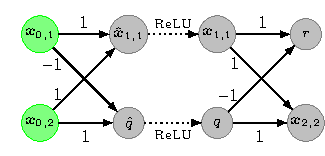
\includegraphics[width=4.5cm]{images/net_no_bounds.pdf}};
%\node [fig, fill=white, right of=1, xshift=8.25em, line width=0.025cm] (1) {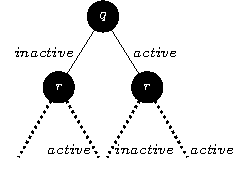
\includegraphics[width=3cm]{images/tree_no_cross.pdf}};
%\end{tikzpicture}
%\end{figure}


	%\item Computation of pre-activation bounds

    %\item Intra- and inter-layer dependency identification procedures

	%\item Translation dependencies into MILP constraints 
	%\item Extension of the underlying MILP program with dependency constraints
%\end{itemize}

%\blfootnote{E. Botoeva, {\bf P. Kouvaros}, J. Kronqvist, R. Misener. {\em Efficient Verification of ReLU-based Neural Networks via Dependency Analyis.} AAAI20}
%\end{frame}

%%%%%%%%%%%%%%%%%%%%%%%%%%%%%%%%%%%%%%%%%%%%%%%%%%%%%%%%%%%%%%%%%%%%%%%%%%%%%%

%\begin{frame}{Dependency analysis}

%\begin{itemize} \itemsep 1em

	%\item Snapshot of the branch-and-bound tree
	
    %\item {\bf Computation of pre-activation bounds}

%\begin{figure}
%\begin{tikzpicture}
%\node [fig, fill=white, line width=0.025cm] (1) {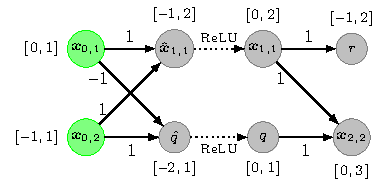
\includegraphics[width=4.5cm]{images/net_bounds_no_edge.pdf}};
%\node [fig, fill=white, right of=1, xshift=8.25em, line width=0.025cm] (1) {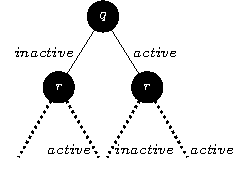
\includegraphics[width=3cm]{images/tree_no_cross.pdf}};
%\end{tikzpicture}
%\end{figure}


    %\item Intra- and inter-layer dependency identification procedures

	%\item Translation dependencies into MILP constraints 
	%\item Extension of the underlying MILP program with dependency constraints
%\end{itemize}

%\blfootnote{E. Botoeva, {\bf P. Kouvaros}, J. Kronqvist, R. Misener. {\em Efficient Verification of ReLU-based Neural Networks via Dependency Analyis.} AAAI20}
%\end{frame}

%%%%%%%%%%%%%%%%%%%%%%%%%%%%%%%%%%%%%%%%%%%%%%%%%%%%%%%%%%%%%%%%%%%%%%%%%%%%%

%\begin{frame}{Dependency analysis}

%\begin{itemize} \itemsep 1em

	%\item Snapshot of the branch-and-bound tree
	
    %\item Computation of pre-activation bounds

    %\item {\bf Intra- and inter-layer dependency identification procedures}

%\begin{figure}
%\begin{tikzpicture}
%\node [fig, fill=white, line width=0.025cm] (1) {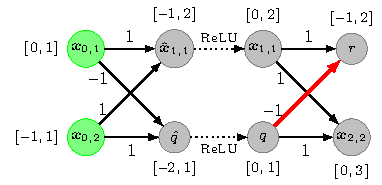
\includegraphics[width=4.5cm]{images/net_bounds.pdf}};
%\node [fig, fill=white, right of=1, xshift=11em, line width=0.025cm] (1) {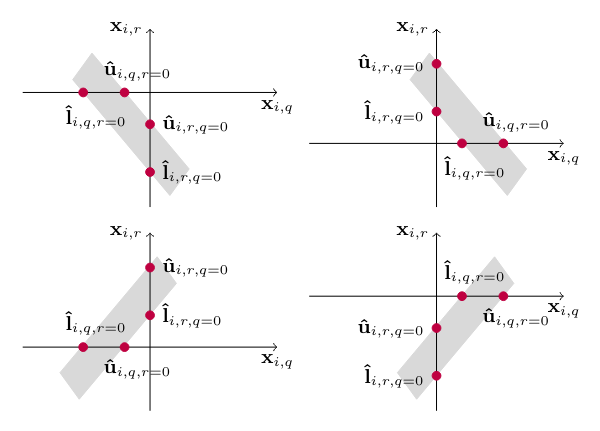
\includegraphics[width=4.75cm]{images/deps.png}};
%\end{tikzpicture}
%\end{figure}

	%\item Translation dependencies into MILP constraints 
	%\item Extension of the underlying MILP program with dependency constraints
%\end{itemize}

%\blfootnote{E. Botoeva, {\bf P. Kouvaros}, J. Kronqvist, R. Misener. {\em Efficient Verification of ReLU-based Neural Networks via Dependency Analyis.} AAAI20}
%\end{frame}

%%%%%%%%%%%%%%%%%%%%%%%%%%%%%%%%%%%%%%%%%%%%%%%%%%%%%%%%%%%%%%%%%%%%%%%%%%%%%

%\begin{frame}{Dependency analysis}

%\begin{itemize} \itemsep 1.5em

	%\item Snapshot of the branch-and-bound tree
	
    %\item Computation of pre-activation bounds

    %\item Intra- and inter-layer dependency identification procedures

    %\item {\bf Translation dependencies into MILP constraints}

%\begin{figure}
%\begin{tikzpicture}
    %\node [fig, fill=white, line width=0.025cm] (1) {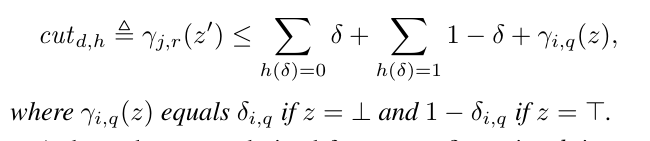
\includegraphics[width=5.5cm]{images/cuts.png}};
%\end{tikzpicture}
%\end{figure}
	%\item Extension of the underlying MILP program with dependency constraints

%\end{itemize}

%\blfootnote{E. Botoeva, {\bf P. Kouvaros}, J. Kronqvist, R. Misener. {\em Efficient Verification of ReLU-based Neural Networks via Dependency Analyis.} AAAI20}
%\end{frame}

%%%%%%%%%%%%%%%%%%%%%%%%%%%%%%%%%%%%%%%%%%%%%%%%%%%%%%%%%%%%%%%%%%%%%%%%%%%%%

%\begin{frame}{Dependency analysis}

%\begin{itemize} \itemsep 1em

	%\item Snapshot of the branch-and-bound tree
	
    %\item Computation of pre-activation bounds

    %\item Intra- and inter-layer dependency identification procedures

	%\item Translation dependencies into MILP constraints 
    %\item {\bf Extension of the underlying MILP program with dependency constraints}

        %\begin{itemize}
            %\item[\textcolor{black}{-}] If node~$q$ becomes inactive, then
                %node~$r$ has to be active; {\bf $r$ depends on $q$}


%\begin{figure}
%\begin{tikzpicture}
%\node [fig, fill=white, line width=0.025cm] (1) {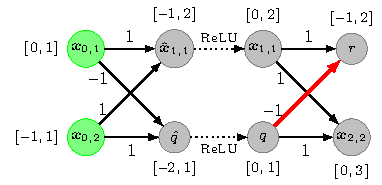
\includegraphics[width=4.4cm]{images/net_bounds.pdf}};
%\node [fig, fill=white, right of=1, xshift=8.75em, line width=0.025cm] (1) {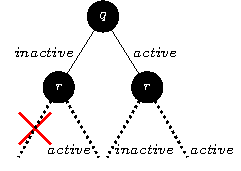
\includegraphics[width=3cm]{images/tree_cross.pdf}};
%\end{tikzpicture}
%\end{figure}


    %\end{itemize}

%\end{itemize}

%\blfootnote{E. Botoeva, {\bf P. Kouvaros}, J. Kronqvist, R. Misener. {\em Efficient Verification of ReLU-based Neural Networks via Dependency Analyis.} AAAI20}
%\end{frame}

%%%%%%%%%%%%%%%%%%%%%%%%%%%%%%%%%%%%%%%%%%%%%%%%%%%%%%%%%%%%%%%%%%%%%%%%%%%%%

%\begin{frame}{Dependency-based branching}

%\begin{itemize} \itemsep 1em

    %\item Dependency-based {\bf heuristic} for selecting the ReLU node to branch

    %\begin{itemize} \itemsep 1em
        %\item[\textcolor{black}{-}] Identification of node dependencies

%\begin{figure}
%\begin{tikzpicture}
%\node [fig, fill=white, line width=0.025cm] (1) {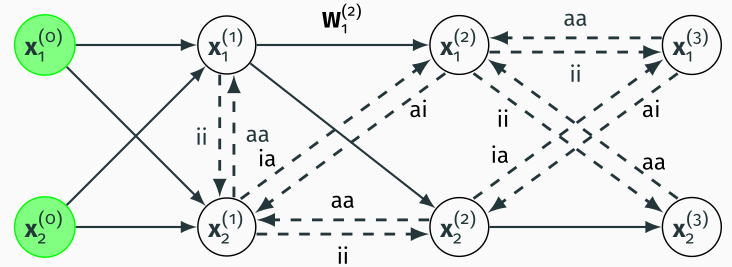
\includegraphics[width=4.4cm]{images/depbranch1.png}};
%\end{tikzpicture}
%\end{figure}
        %\item[\textcolor{black}{-}] Construction of the dependency graph
%\begin{figure}
%\begin{tikzpicture}
%\node [fig, fill=white, line width=0.025cm] (1) {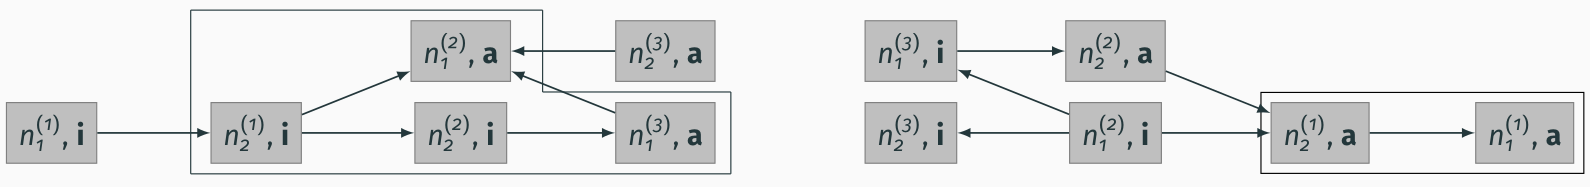
\includegraphics[width=8.5cm]{images/depbranch2.png}};
%\end{tikzpicture}
%\end{figure}
        %\item[\textcolor{black}{-}] Selection of the node with the most nodes dependent on it
	%\end{itemize}


    %\item Division of the verification problem into sub-problems with simpler MILP-formulations (i.e., with fewer binary variables)
	

%\end{itemize}

%\blfootnote{{\bf P. Kouvaros}, A. Lomsucio. {\em Towards Scalable Complete Verification of ReLU Neural Networks via Dependency-based Branching}. IJCAI21}


%\end{frame}

%%%%%%%%%%%%%%%%%%%%%%%%%%%%%%%%%%%%%%%%%%%%%%%%%%%%%%%%%%%%%%%%%%%%%%%%%%%%%

\begin{frame}{\texttt{{\bf Venus}}}

\begin{itemize}  \itemsep 1em
    \item Open-source neural network verification tool 

    \item Extensive support for various types of layers and architectures
        present in applications
    
    \item Advances in symbolic bound propagation,
        dependency analysis and input domain splitting

    \item From checking networks of thoundands of nodes in 2019 it has
        progressed to the verification of networks of millions of nodes in 2023
    \vspace{1em}
    \begin{figure}
    \begin{tikzpicture}
        \node [fig, fill=white, line width=0.025cm] (1) {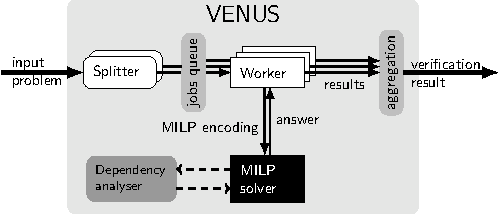
\includegraphics[width=5.5cm]{images/venus2.pdf}};
        %\node [fig, fill=white, line width=0.025cm, right of=1, xshift=11em] (1) {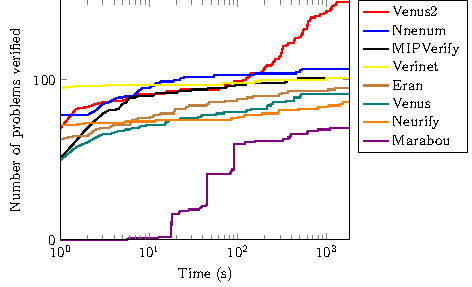
\includegraphics[width=3.9cm]{images/cpmnist.pdf}};
    \end{tikzpicture}
    \end{figure}
\end{itemize}
\end{frame}

%%%%%%%%%%%%%%%%%%%%%%%%%%%%%%%%%%%%%%%%%%%%%%%%%%%%%%%%%%%%%%%%%%%%%%%%%%%%%

%\begin{frame}{Progress in the last four years}
%\begin{itemize} \itemsep 1.5em
        %\item {\bf Experimental progress on ACASXU}
    %\begin{figure}
    %\begin{tikzpicture}
        %\node [fig, fill=white, line width=0.025cm] (1) {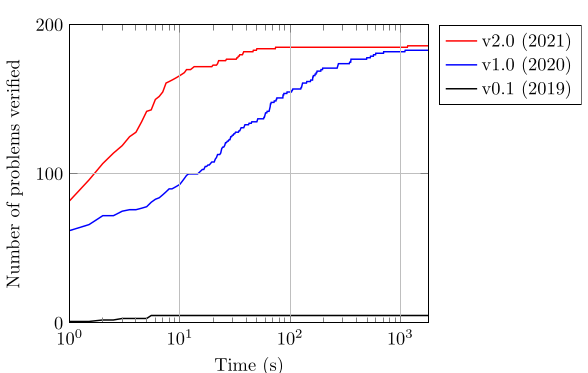
\includegraphics[width=8cm]{images/venus_progress.png}};
    %\end{tikzpicture}
    %\end{figure}

        %\item Architecture support

        %\item Scalability
    %\end{itemize}

%\end{frame}

%%%%%%%%%%%%%%%%%%%%%%%%%%%%%%%%%%%%%%%%%%%%%%%%%%%%%%%%%%%%%%%%%%%%%%%%%%%%%

%\begin{frame}{Progress in the last four years}
    %\begin{itemize}
        %\item  Experimental progress on ACASXU

        %\item {\bf Architecture support}
    %\begin{figure}
    %\begin{tikzpicture}
        %\node [fig, fill=white, line width=0.025cm] (1) {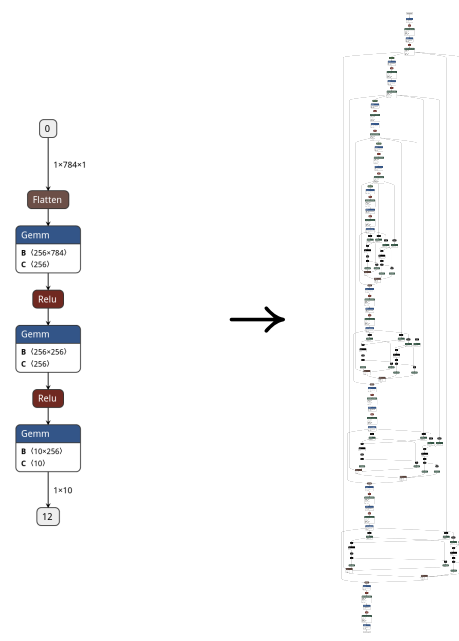
\includegraphics[width=4.7cm]{images/architecture.png}};
    %\end{tikzpicture}
    %\end{figure}

        %\item Scalability
    %\end{itemize}


%\end{frame}

%%%%%%%%%%%%%%%%%%%%%%%%%%%%%%%%%%%%%%%%%%%%%%%%%%%%%%%%%%%%%%%%%%%%%%%%%%%%%

%\begin{frame}{Progress in the last four years}
%\begin{itemize} \itemsep2em
        %\item  Experimental progress on ACASXU

        %\item Architecture support

        %\item {\bf Scalability}
            %\begin{itemize}
                %\item[\textcolor{black}{-}] From networks of thousands of ReLU
                    %nodes in 2018 to networks of millions of nodes in 2023
            %\end{itemize}

    %\begin{figure}
    %\begin{tikzpicture}
        %\node [fig, fill=white, line width=0.025cm] (1) {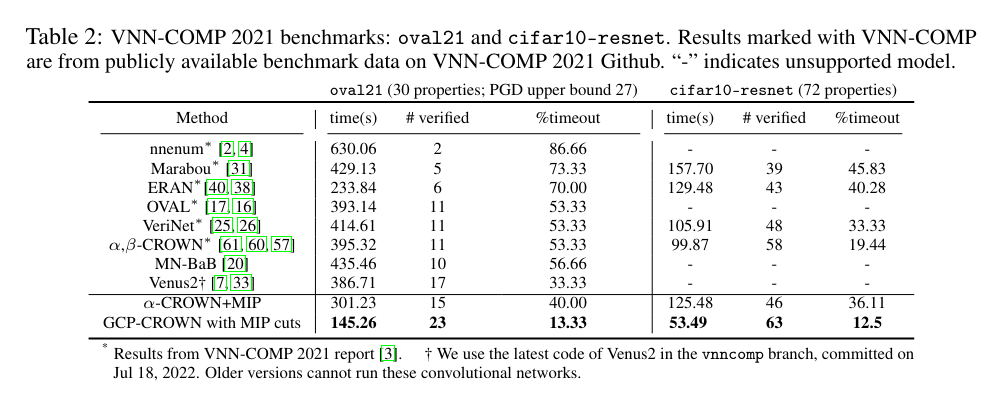
\includegraphics[width=9cm]{images/res1.png}};
    %\end{tikzpicture}
    %\end{figure}
    %\end{itemize}


%\end{frame}

%%%%%%%%%%%%%%%%%%%%%%%%%%%%%%%%%%%%%%%%%%%%%%%%%%%%%%%%%%%%%%%%%%%%%%%%%%%%%

%\begin{frame}{Applications}
%\begin{itemize} \itemsep2em
        %\item  Object detection for autonomous driving (Audi)

        %\item Runway centerline offset detection (Boeing)

        %\item Open category detection (Boeing)
        
        %\item Collision avoidance (Land/Go Around) (Boeing)
        
        %\item Runway key point estimation (Boeing)

    %\end{itemize}
    %\blfootnote{ {\bf P. Kouvaros}, F. Leofante, B. Edwards, C. Chung, D.
    %Margineantu, A. Lomuscio. {\em Verification of Semantic Key Point Detection
    %for Aircraft Pose Estimation}. KR23}
    %\blfootnote{ {\bf P. Kouvaros}, T. Kyono, F. Leofante, A. Lomuscio, D.
    %Margineantu, D. Osipychev, Y. Zheng. {\em Formal Analysis of Neural
    %Network-based Systems in the Aircraft Domain}. FM21}
%\blfootnote{V. Hasemi, {\bf P. Kouvaros}, A. Lomsucio. {\em OSIP: Tightened
    %Bound Propagation for the Verification of ReLU Neural Networks}. SEFM21}
%\end{frame}

%%%%%%%%%%%%%%%%%%%%%%%%%%%%%%%%%%%%%%%%%%%%%%%%%%%%%%%%%%%%%%%%%%%%%%%%%%%%%


\begin{frame}{Runway Detection}
\begin{itemize}

    \item {\bf Challenge:} Key point prediction robustness: Is the key point prediction robust against input perturbations?
        %\item[\textcolor{black}{-}]  Variability in key point confidence: What
            %is the degree of change to the confidence of a key point prediction
            %under input perturbations?
    \item {\bf Models:} U-Nets with approximately 2 million non-linear nodes
    \item {\bf Input perturbations}: white noise in (segments of) the input and photometric changes, including brightness and contrast changes
    \vspace{1em}
    \begin{figure}
    \begin{tikzpicture}
        \node [fig, fill=white, line width=0.025cm] (1) {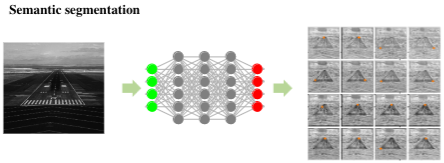
\includegraphics[width=5cm]{images/pnp1.png}};
        \node [fig, fill=white, line width=0.025cm, right of=1, xshift=4cm] (1) {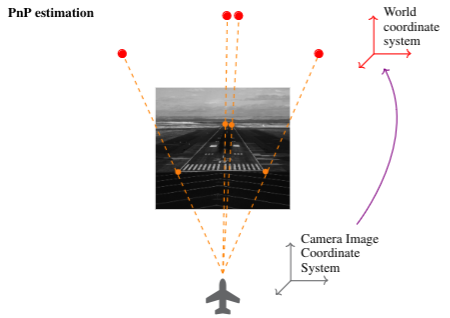
\includegraphics[width=4.5cm]{images/pnp2.png}};
    \end{tikzpicture}
    \end{figure}

    \end{itemize}

\end{frame}

%%%%%%%%%%%%%%%%%%%%%%%%%%%%%%%%%%%%%%%%%%%%%%%%%%%%%%%%%%%%%%%%%%%%%%%%%%%%%

\begin{frame}{Runway Detection --- Analysis Summary}
\begin{itemize}
    \item The models are robust with respect to minor perturbations but still
        {\bf brittle to realistic alterations of the input}
\item The models are more susceptible to some variabilities (brightness) than
others (contrast)
%\item The models can be augmented with \texttt{Venus} counterexamples or  adversarially trained
\end{itemize}
\begin{figure}
\begin{tikzpicture}
    %\node [fig, fill=white, line width=0.025cm, label={Brightness results}] (1) {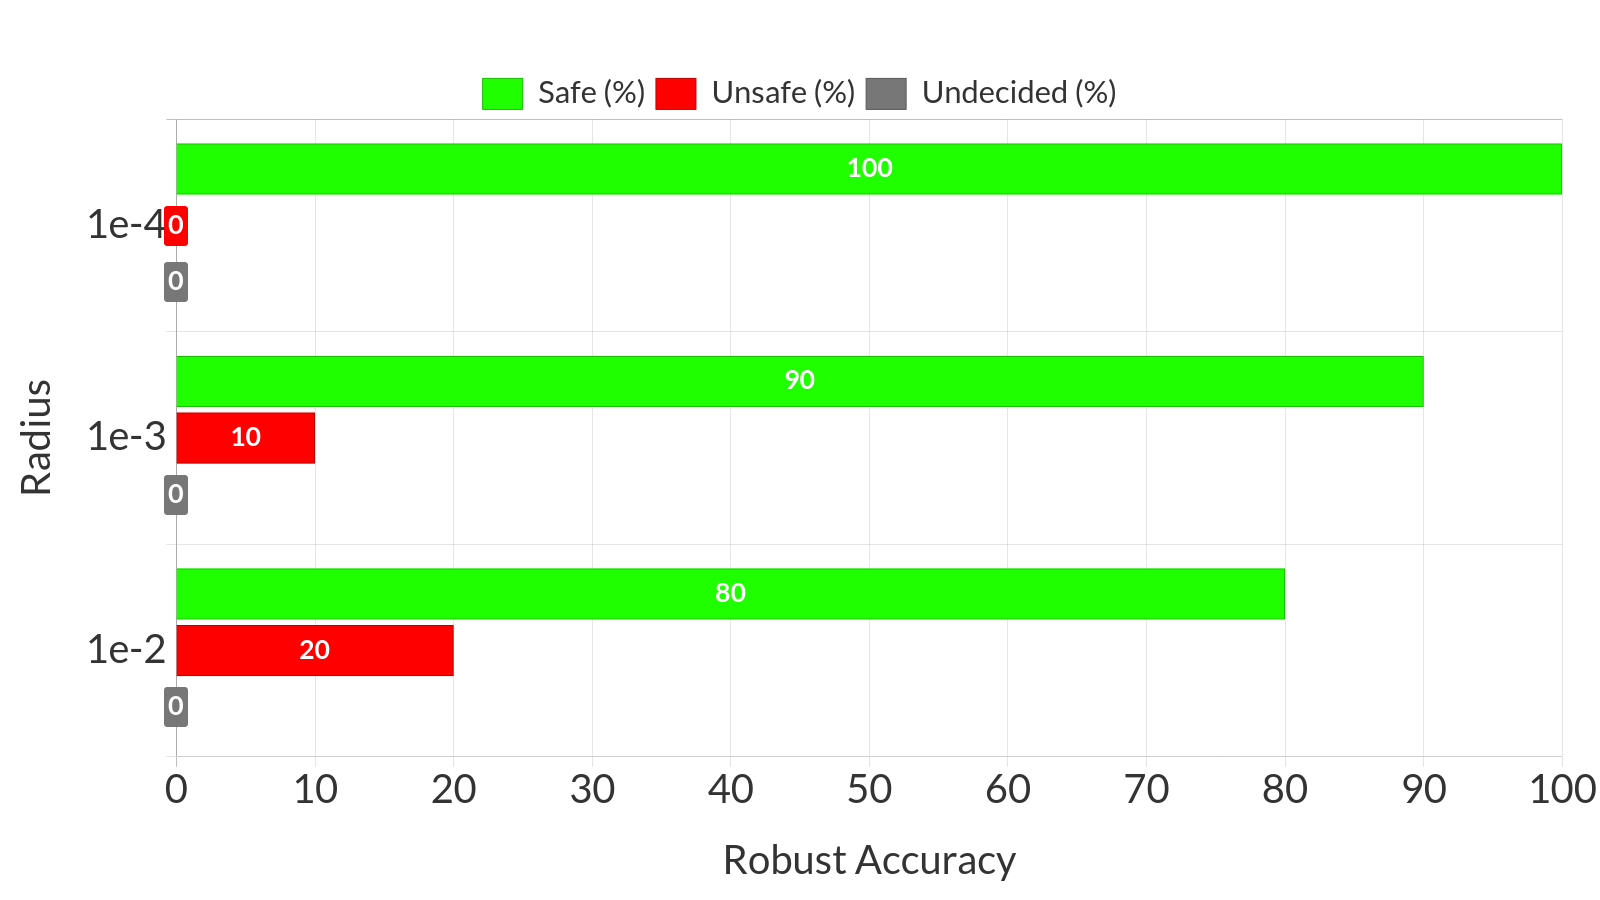
\includegraphics[width=4.5cm]{images/brightness.png}};
        \node [fig, fill=white, line width=0.025cm, right of=1, xshift=9em, label={Original}] (2) {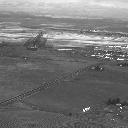
\includegraphics[width=3cm]{images/cex.jpg}};
        \node [fig, fill=white, line width=0.025cm, right of=2, xshift=5em, label={Counterexample}] (3) {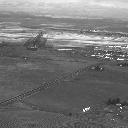
\includegraphics[width=3cm]{images/cex.jpg}};
    \end{tikzpicture}
    \end{figure}

\end{frame}


%%%%%%%%%%%%%%%%%%%%%%%%%%%%%%%%%%%%%%%%%%%%%%%%%%%%%%%%%%%%%%%%%%%%%%%%%%%%%

\begin{frame}{Verification of Neuro-symbolic Multi-agent Systems}

%\begin{itemize} \itemsep 2em 
        %\item \textcolor{Charcoal}{{\bf Unbounded multi-agent systems}  (decentralised systems with
		%arbitrarily many symbolic participants, e.g., robot swarms)}

    %\item {\bf Neuro-symbolic multi-agent systems} (e.g., autonomous vehicles)

    \begin{figure}
        \begin{tikzpicture}
        \node [fig, fill=white, line width=0.025cm] (1) {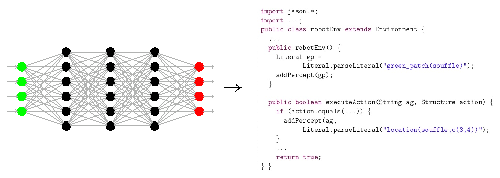
\includegraphics[width=9cm]{images/neurosymagent.pdf}};
        \end{tikzpicture}
        \end{figure}

    %\item \textcolor{Charcoal}{Standalone {\bf neural agents} (e.g., perception)}

%\end{itemize}

\end{frame}



%%%%%%%%%%%%%%%%%%%%%%%%%%%%%%%%%%%%%%%%%%%%%%%%%%%%%%%%%%%%%%%%%%%%%%%%%%%%%%

%\begin{frame}{Neural-symbolic Multi-agent Systems}



%\begin{center}
%%\documentclass{standalone}

\usepackage[T1]{fontenc}
\usepackage{amsmath,amssymb,mathtools}
\newcommand{\set}[1]{\left\{ #1 \right \}}

\usepackage{graphicx}
\definecolor{navyblue}{RGB}{0,0,128}

\begin{document}

	\begin{tikzpicture}[ font=\scriptsize] 

	 \node[] (0)
	 {\scalebox{0.5}{\begin{tikzpicture}[node distance=0.5cm,
	font=\scriptsize,auto,
	every node/.style={circle,inner sep=0.1cm},
	input/.style={fill=green,draw=green},
	hidden/.style={fill=black,draw=black},
	output/.style={fill=red,draw=red}]

  
  \node [input] (i1) {};
  \node [below of=i1, input] (i2) {};
  \node [below of=i2, input] (i3) {};
  \node [below of=i3, input] (i4) {};

  \node [right of = i1, above of = i1, xshift=1cm, hidden] (h11) {};
  \node [below of=h11, hidden] (h12) {};
  \node [below of=h12, hidden] (h13) {};
  \node [below of=h13, hidden] (h14) {};
  \node [below of=h14, hidden] (h15) {};
  \node [below of=h15, hidden] (h16) {};

  \node [right of = h11, xshift=1cm, hidden] (h21) {};
  \node [below of=h21, hidden] (h22) {};
  \node [below of=h22, hidden] (h23) {};
  \node [below of=h23, hidden] (h24) {};
  \node [below of=h24, hidden] (h25) {};
  \node [below of=h25, hidden] (h26) {};

  \node [right of = h21, xshift=1cm, hidden] (h31) {};
  \node [below of=h31, hidden] (h32) {};
  \node [below of=h32, hidden] (h33) {};
  \node [below of=h33, hidden] (h34) {};
  \node [below of=h34, hidden] (h35) {};
  \node [below of=h35, hidden] (h36) {};

  \node [right of = h32, xshift=1cm, output] (o1) {};
  \node [below of=o1, output] (o2) {};
  \node [below of=o2, output] (o3) {};
  \node [below of=o3, output] (o4) {};
  %\node [right of=1, xshift=-1.52m, fill=gray!50!white,draw=gray,neuron] (3) {};

  \foreach \i in {1,...,4}{
	  \draw[<-,color=black!30!white] (i\i) -- ++(-0.5,0);
	  \draw[->,color=black!30!white] (o\i) -- ++(0.5,0);
  }
  \foreach \i in {1,...,4}{
	 \foreach \j in {1,...,6}{
		 \draw [color=black!30!white]  (i\i) -- (h1\j);
   }}
  \foreach \i in {1,...,6}{
	 \foreach \j in {1,...,6}{
		 \draw [color=black!30!white]  (h1\i) -- (h2\j);
		 \draw [color=black!30!white]  (h2\i) -- (h3\j);
   }}
  \foreach \i in {1,...,6}{
	 \foreach \j in {1,...,4}{
		 \draw [color=black!30!white]  (h3\i) -- (o\j);
   }}

   %\node[below of=h16,xshift=-1cm,yshift=-0.5cm,input,label=right:{input node}] (inf1) {};
   %\node[right of=inf1,xshift=1.5cm,hidden,label=right:{hidden node}] (inf2) {};
   %\node[right of=inf2,xshift=1.5cm,output,label=right:{output node}] (inf3) {};

\end{tikzpicture}
}};

	 \node[right of = 0,xshift=3em] (1) (1) { {\large $\rightarrow$}};
	 \node[right of = 1,xshift=4em] (2) {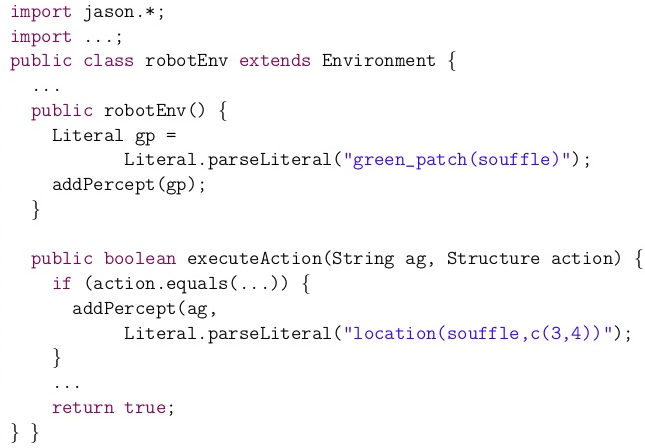
\includegraphics[width=4cm]{program.png}};

	%\draw[draw=black,rounded corners] (-1.3,-1) rectangle ++(3,2.2);	
	%\draw[draw=black,rounded corners] (-1.2,-0.9) rectangle ++(2.8,2);	
	%\draw[draw=black,rounded corners] (-1.6,-0.5) rectangle ++(0.3,1);	
	%\draw[draw=black,rounded corners] (1.7,-0.5) rectangle ++(0.3,1);	
	
		%\node[draw=navyblue,rectangle,inner
		%sep=0.2cm, fit=(0)(1)(2)] {};
	

  \end{tikzpicture}

\end{document}




%\end{center}

%\textbf{Neural-symbolic} agents are equipped with
  %\begin{itemize}
  %\item a \textbf{neural}-based perception unit, e.g., a ReLU-based
	%feed-forward neural network
  %\item a \textbf{symbolic} controller unit, e.g., modelled via
	%concurrent-game structures, or interpreted systems.
  %\end{itemize}

%\end{frame}

%%%%%%%%%%%%%%%%%%%%%%%%%%%%%%%%%%%%%%%%%%%%%%%%%%%%%%%%%%%

\begin{frame}{Neuro-symbolic Multi-agent Systems}

\begin{itemize} \itemsep 1em
    \item Agents are equipped with a neural perception unit and a symbolic
        controller
    \item {\bf } A {\bf neuro-symbolic agent} is a tuple $\tuple{\Loc_a,
        \obs_a, \Act_a, \prot_a, \tran_a}$, where

        \begin{itemize}\itemsep 0cm
            \item[\textcolor{black}{-}] $\Loc_a = \Prv_a\times\Per_a$ is a
                \emph{set of local states} comprising tuples of {\em private
                states} and {\em percepts}
            \item[\textcolor{black}{-}]
                $\obs_a\colon\Loc_a\times\Loc_\env\rightarrow\Per_a$ is an
                \emph{observation function} implemented by a neural network
            \item[\textcolor{black}{-}] $\Act_a$ is a nonempty finite \emph{set
                of actions}
            \item[\textcolor{black}{-}] $\prot_a\colon\Loc_a\rightarrow
                2^{\Act_a}\setminus \emptyset$ is a {\em local protocol
                function}
            \item[\textcolor{black}{-}]
                $\tran_a\colon\Loc_a\times\Act_1\times\dots\times\Act_\maxagt\times\Act_\env\rightarrow\Prv_a$
                is a {\em local transition function}
        \end{itemize}

\end{itemize}
    \vspace{1em}
    \begin{figure}
    
\begin{tikzpicture}
        \node[rectangle, color=white, fill=black, minimum height=2em] (1) {{\scriptsize private}};
        \node[rectangle, color=white, fill=red, right of=1, minimum height=2em] {{\scriptsize percept}};
    \end{tikzpicture}
    \end{figure}


    %\blfootnote{M. Akintunde, E. Botoeva, {\bf P. Kouvaros}, A. Lomsucio. {{\em  Verifying Strategic Abilities of Neural-symbolic Multi-agent Systems}}. KR20}


\end{frame}

%%%%%%%%%%%%%%%%%%%%%%%%%%%%%%%%%%%%%%%%%%%%%%%%%%%%%%%%%%%

\begin{frame}{Neuro-symbolic Multi-agent Systems}

\begin{itemize} \itemsep 1em
    \item Agents are equipped with a neural perception unit and a symbolic
        controller
    \item {\bf } A {\bf neuro-symbolic agent} is a tuple $\tuple{\Loc_a,
        \obs_a, \Act_a, \prot_a, \tran_a}$, where

        \begin{itemize}\itemsep 0cm
            \item[\textcolor{black}{-}] $\Loc_a = \Prv_a\times\Per_a$ is a
                \emph{set of local states} comprising tuples of {\em private
                states} and {\em percepts}
            \item[\textcolor{black}{-}]
                $\obs_a\colon\Loc_a\times\Loc_\env\rightarrow\Per_a$ is an
                \emph{observation function} implemented by a neural network
            \item[\textcolor{black}{-}] $\Act_a$ is a nonempty finite \emph{set
                of actions}
            \item[\textcolor{black}{-}] $\prot_a\colon\Loc_a\rightarrow
                2^{\Act_a}\setminus \emptyset$ is a {\em local protocol
                function}
            \item[\textcolor{black}{-}]
                $\tran_a\colon\Loc_a\times\Act_1\times\dots\times\Act_\maxagt\times\Act_\env\rightarrow\Prv_a$
                is a {\em local transition function}
        \end{itemize}

\end{itemize}
    \vspace{1em}
    \begin{figure}
    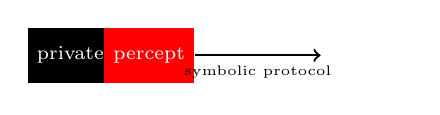
\begin{tikzpicture}
        \node[rectangle, color=white, fill=black, minimum height=2em] (1) {{\scriptsize private}};
        \node[rectangle, color=white, fill=red, right of=1, minimum height=2em] (2) {{\scriptsize percept}};
        \node[rectangle, color=white, fill=white, right of=2, minimum height=2em, xshift=5em] (3) {{\scriptsize percept}};

        \path[->, thick, align=left]  (2) edge node[below] {{\tiny symbolic protocol}} (3);
    \end{tikzpicture}

    \end{figure}

    %\blfootnote{M. Akintunde, E. Botoeva, {\bf P. Kouvaros}, A. Lomsucio. {{\em  Verifying Strategic Abilities of Neural-symbolic Multi-agent Systems}}. KR20}


\end{frame}


%%%%%%%%%%%%%%%%%%%%%%%%%%%%%%%%%%%%%%%%%%%%%%%%%%%%%%%%%%%

\begin{frame}{Neuro-symbolic Multi-agent Systems}

\begin{itemize} \itemsep 1em
    \item Agents are equipped with a neural perception unit and a symbolic
        controller
    \item {\bf } A {\bf neuro-symbolic agent} is a tuple $\tuple{\Loc_a,
        \obs_a, \Act_a, \prot_a, \tran_a}$, where

        \begin{itemize}\itemsep 0cm
            \item[\textcolor{black}{-}] $\Loc_a = \Prv_a\times\Per_a$ is a
                \emph{set of local states} comprising tuples of {\em private
                states} and {\em percepts}
            \item[\textcolor{black}{-}]
                $\obs_a\colon\Loc_a\times\Loc_\env\rightarrow\Per_a$ is an
                \emph{observation function} implemented by a neural network
            \item[\textcolor{black}{-}] $\Act_a$ is a nonempty finite \emph{set
                of actions}
            \item[\textcolor{black}{-}] $\prot_a\colon\Loc_a\rightarrow
                2^{\Act_a}\setminus \emptyset$ is a {\em local protocol
                function}
            \item[\textcolor{black}{-}]
                $\tran_a\colon\Loc_a\times\Act_1\times\dots\times\Act_\maxagt\times\Act_\env\rightarrow\Prv_a$
                is a {\em local transition function}
        \end{itemize}

\end{itemize}
    \vspace{1em}
    \begin{figure}
    
\begin{tikzpicture}
        \node[rectangle, color=white, fill=black, minimum height=2em] (1) {{\scriptsize private}};
        \node[rectangle, color=white, fill=red, right of=1, minimum height=2em] (2) {{\scriptsize percept}};
        \node[rectangle, color=white, fill=white, right of=2, minimum height=2em, xshift=5em] (3) {{\scriptsize percept}};

        \path[->, thick, align=left]  (2) edge node[above] {{\tiny action}} (3);
    \end{tikzpicture}

    \end{figure}

    %\blfootnote{M. Akintunde, E. Botoeva, {\bf P. Kouvaros}, A. Lomsucio. {{\em  Verifying Strategic Abilities of Neural-symbolic Multi-agent Systems}}. KR20}


\end{frame}

%%%%%%%%%%%%%%%%%%%%%%%%%%%%%%%%%%%%%%%%%%%%%%%%%%%%%%%%%%%

\begin{frame}{Neuro-symbolic Multi-agent Systems}

\begin{itemize} \itemsep 1em
    \item Agents are equipped with a neural perception unit and a symbolic
        controller
    \item {\bf } A {\bf neuro-symbolic agent} is a tuple $\tuple{\Loc_a,
        \obs_a, \Act_a, \prot_a, \tran_a}$, where

        \begin{itemize}\itemsep 0cm
            \item[\textcolor{black}{-}] $\Loc_a = \Prv_a\times\Per_a$ is a
                \emph{set of local states} comprising tuples of {\em private
                states} and {\em percepts}
            \item[\textcolor{black}{-}]
                $\obs_a\colon\Loc_a\times\Loc_\env\rightarrow\Per_a$ is an
                \emph{observation function} implemented by a neural network
            \item[\textcolor{black}{-}] $\Act_a$ is a nonempty finite \emph{set
                of actions}
            \item[\textcolor{black}{-}] $\prot_a\colon\Loc_a\rightarrow
                2^{\Act_a}\setminus \emptyset$ is a {\em local protocol
                function}
            \item[\textcolor{black}{-}]
                $\tran_a\colon\Loc_a\times\Act_1\times\dots\times\Act_\maxagt\times\Act_\env\rightarrow\Prv_a$
                is a {\em local transition function}
        \end{itemize}

\end{itemize}
    \vspace{1em}
    \begin{figure}
    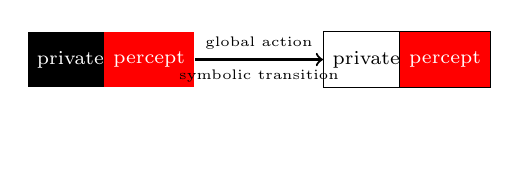
\begin{tikzpicture}
        \node[rectangle, color=white, fill=black, minimum height=2em] (1) {{\scriptsize private}};
        \node[rectangle, color=white, fill=red, right of=1, minimum height=2em] (2) {{\scriptsize percept}};
        \node[rectangle, fill=white, draw=black, right of=2, minimum height=2em, xshift=5em] (3) {{\scriptsize private}};
        \node[rectangle, color=white, fill=red, draw=black, right of=3, minimum height=2em] (4) {{\scriptsize percept}};

        \node[below of=3] (5) {};

        \path[->, thick, align=left]  
        (2) edge node[above] {{\tiny global action}} node[below] {{\tiny symbolic transition}} (3);
        %(5) edge node[right] {{\tiny other actions}} (3);
    \end{tikzpicture}

    \end{figure}

    %\blfootnote{M. Akintunde, E. Botoeva, {\bf P. Kouvaros}, A. Lomsucio. {{\em  Verifying Strategic Abilities of Neural-symbolic Multi-agent Systems}}. KR20}


\end{frame}

%%%%%%%%%%%%%%%%%%%%%%%%%%%%%%%%%%%%%%%%%%%%%%%%%%%%%%%%%%%


\begin{frame}{Neuro-symbolic Multi-agent Systems}

\begin{itemize} \itemsep 1em
    \item Agents are equipped with a neural perception unit and a symbolic
        controller
    \item {\bf } A {\bf neuro-symbolic agent} is a tuple $\tuple{\Loc_a,
        \obs_a, \Act_a, \prot_a, \tran_a}$, where

        \begin{itemize}\itemsep 0cm
            \item[\textcolor{black}{-}] $\Loc_a = \Prv_a\times\Per_a$ is a
                \emph{set of local states} comprising tuples of {\em private
                states} and {\em percepts}
            \item[\textcolor{black}{-}]
                $\obs_a\colon\Loc_a\times\Loc_\env\rightarrow\Per_a$ is an
                \emph{observation function} implemented by a neural network
            \item[\textcolor{black}{-}] $\Act_a$ is a nonempty finite \emph{set
                of actions}
            \item[\textcolor{black}{-}] $\prot_a\colon\Loc_a\rightarrow
                2^{\Act_a}\setminus \emptyset$ is a {\em local protocol
                function}
            \item[\textcolor{black}{-}]
                $\tran_a\colon\Loc_a\times\Act_1\times\dots\times\Act_\maxagt\times\Act_\env\rightarrow\Prv_a$
                is a {\em local transition function}
        \end{itemize}

\end{itemize}
    \vspace{1em}
    \begin{figure}
    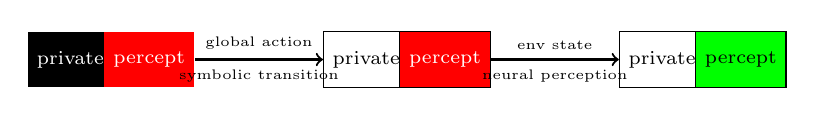
\begin{tikzpicture}
        \node[rectangle, color=white, fill=black, minimum height=2em] (1) {{\scriptsize private}};
        \node[rectangle, color=white, fill=red, right of=1, minimum height=2em] (2) {{\scriptsize percept}};
        \node[rectangle, fill=white, draw=black, right of=2, minimum height=2em, xshift=5em] (3) {{\scriptsize private}};
        \node[rectangle, color=white, fill=red, draw=black, right of=3, minimum height=2em] (4) {{\scriptsize percept}};

        \node[rectangle, fill=white, draw=black, right of=4, minimum height=2em, xshift=5em] (6) {{\scriptsize private}};
        \node[rectangle, fill=green, draw=black, right of=6, minimum height=2em] (7) {{\scriptsize percept}};


        \path[->, thick, align=left]  
        (2) edge node[above] {{\tiny global action}} node[below] {{\tiny symbolic transition}} (3)
        (4) edge node[above] {\tiny{env state}} node[below] {{\tiny neural perception}} (6);
    \end{tikzpicture}

    \end{figure}
    

%\blfootnote{M. Akintunde, E. Botoeva, {\bf P. Kouvaros}, A. Lomsucio. {{\em  Verifying Strategic Abilities of Neural-symbolic Multi-agent Systems}}. KR20}



\end{frame}



%%%%%%%%%%%%%%%%%%%%%%%%%%%%%%%%%%%%%%%%%%%%%%%%%%%%%%%%%%%

\begin{frame}{Neuro-symbolic Multi-agent Systems}

\begin{itemize} \itemsep 1em
    \item Agents are equipped with a neural perception unit and a symbolic
        controller
    \item {\bf } A {\bf neuro-symbolic agent} is a tuple $\tuple{\Loc_a,
        \obs_a, \Act_a, \prot_a, \tran_a}$, where

        \begin{itemize}\itemsep 0cm
            \item[\textcolor{black}{-}] $\Loc_a = \Prv_a\times\Per_a$ is a
                \emph{set of local states} comprising tuples of {\em private
                states} and {\em percepts}
            \item[\textcolor{black}{-}]
                $\obs_a\colon\Loc_a\times\Loc_\env\rightarrow\Per_a$ is an
                \emph{observation function} implemented by a neural network
            \item[\textcolor{black}{-}] $\Act_a$ is a nonempty finite \emph{set
                of actions}
            \item[\textcolor{black}{-}] $\prot_a\colon\Loc_a\rightarrow
                2^{\Act_a}\setminus \emptyset$ is a {\em local protocol
                function}
            \item[\textcolor{black}{-}]
                $\tran_a\colon\Loc_a\times\Act_1\times\dots\times\Act_\maxagt\times\Act_\env\rightarrow\Prv_a$
                is a {\em local transition function}
        \end{itemize}

    \item {\bf Environments} are similarly defined (but no percepts)
    
    \item {\bf Neuro-symbolic MAS} compose neuro-symbolic agents with the environment for a set $I$ of initial states
\end{itemize}

%\blfootnote{M. Akintunde, E. Botoeva, {\bf P. Kouvaros}, A. Lomsucio. {{\em  Verifying Strategic Abilities of Neural-symbolic Multi-agent Systems}}. KR20}
\end{frame}

%%%%%%%%%%%%%%%%%%%%%%%%%%%%%%%%%%%%%%%%%%%%%%%%%%%%%%%%%%%

\begin{frame}{Formal Verification of NMAS}

\begin{itemize} \itemsep 1.5em
    \item {\bf Verification problem}: Given a NMAS $\mathcal S$ and a logic formula 
	   $\varphi$, check whether every initial state in $\mathcal S$ satisfies $\varphi$
    \item  Verification of NMAS against unbounded reachability properties
        (i.e., the system eventually reaches an unsafe state) is
        {\bf undecidable}
    \item Bounded fragment of {\bf ATL$^*$} (alternating-time temporal logic):
  \[\begin{array}{rcl} \varphi \! \! \!  & ::= \!  \!  \!
      & \red{\alpha} \mid \varphi \lor \varphi \mid \varphi \land \varphi \mid
	  \red{\egamma{k} \varphi, \mid [[\Gamma]]^k \varphi} %\mid \agamma{k} \varphi},
      % \mid E(\varphi U^k \varphi) \mid A(\varphi U^k \varphi),
      \\
      \alpha \! \! \!  & ::= \!  \!  \!
      & c_1(1)+\cdots+c_m(m) \op c
    \end{array}\]
    where $\alpha$ is a linear inequality over the outputs of the network and 
    $\agt$ is a subset of agents.
        \vspace{1em}

        \begin{itemize}
            \item[\textcolor{black}{-}] $\egamma[ag]{k} (\text{safe})$: ``agent
                $ag$ has a strategy to enter a safe configuration after $k$
                steps irrespective of what the intruder does.''
        \end{itemize}
    \end{itemize}

%\blfootnote{M. Akintunde, E. Botoeva, {\bf P. Kouvaros}, A. Lomsucio. {{ \em
    %Formal Verification of Neural Agents in Non-determenistic Environments}}.
    %AAMAS20}

%\blfootnote{M. Akintunde, E. Botoeva, {\bf P. Kouvaros}, A. Lomsucio. {{\em  Verifying Strategic Abilities of Neural-symbolic Multi-agent Systems}}. KR20}

\end{frame}


%%%%%%%%%%%%%%%%%%%%%%%%%%%%%%%%%%%%%%%%%%%%%%%%%%%%%%%%%%%

\begin{frame}{MILP Encodings}

\begin{itemize} \itemsep 1em
        \item The verification problem is recast to a {\bf MILP feasibility problem}

    \item {\bf Monolithic} encoding
        \begin{itemize}
            \item[\textcolor{black}{-}] $\mathcal S \models \varphi$ iff
                $\pi_{\mathcal S, \neg \varphi \land \varphi_I}$ is infeasible
            \item[\textcolor{black}{-}] Single (exponentially large) program
                $\pi_{\mathcal S, \neg \varphi \land \varphi_I}$

            \begin{figure}
            \begin{tikzpicture}
            \node [fig] (1) {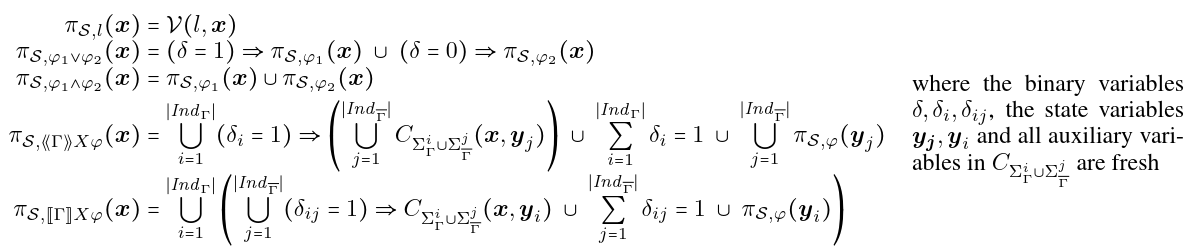
\includegraphics[width=9cm]{images/monolithic.png}};
            \end{tikzpicture}
            \end{figure}
        \end{itemize}

    \item {\bf Compositional} encoding
        \begin{itemize}
            \item[\textcolor{black}{-}] $\mathcal S \models \varphi$ iff
                every program in $\Pi_{\mathcal S, \neg \varphi \land \varphi_I}$ is infeasible
            \item[\textcolor{black}{-}] Set of (smaller) program with parallelisable infeasibility checks

            \begin{figure}
            \begin{tikzpicture}
            \node [fig] (1) {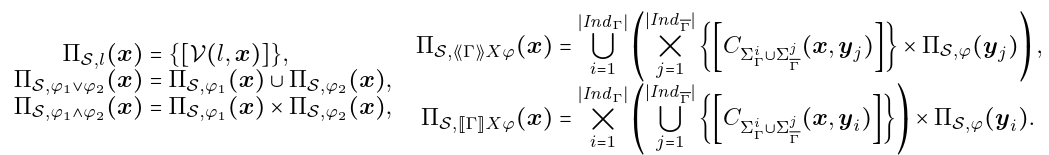
\includegraphics[width=9cm]{images/compositional.png}};
            \end{tikzpicture}
            \end{figure}
        \end{itemize}

\end{itemize} 

%\blfootnote{M. Akintunde, E. Botoeva, {\bf P. Kouvaros}, A. Lomsucio. {{\em  Verifying Strategic Abilities of Neural-symbolic Multi-agent Systems}}. KR20}

\end{frame}

%%%%%%%%%%%%%%%%%%%%%%%%%%%%%%%%%%%%%%%%%%%%%%%%

\begin{frame}{Two-agent Aircraft Collision Avoidance}

  \small
  
  \hspace{-0.6cm}
  \begin{tabular}{@{}l@{~~}l}
    \begin{minipage}{0.71\linewidth}
      \begin{itemize}\itemsep 0.1cm
      \item Two agents, \textbf{ownship} and \textbf{intruder}, each equipped
        with a \textbf{collision avoidance system} producing vertical climbrate
        \textbf{advisories} to the pilot (perception unit).
      \item Given an advisory, the pilot chooses the
        \textbf{acceleration} from an appropriate interval (action
        selection unit).
      \item The goal is to avoid a \textbf{near mid-air collision}
        (NMAC): when the ownship and intruder are separated
        by less than 100ft vertically and 500ft horizontally.

        ~
      \end{itemize}
    \end{minipage}
    &
      \begin{minipage}{0.25\linewidth}\footnotesize
        \begin{tabular}{@{}r@{~~}l}
          $h$:& Vertical separation (ft).\\
          $\crown$:& Ownship vertical\\ &climbrate (ft/s).\\
          $\crint$:& Intruder vertical\\ &climbrate (ft/s).\\
          $\tau$:& Time to loss of\\ &horizontal separation (s).\\
          $\advown$:& Previous advisory\\ &issued to the ownship.\\
          $\advint$:& Previous advisory\\ &issued to the intruder.
        \end{tabular}
      \end{minipage}
                   
  \end{tabular}

    \begin{figure}
    \begin{tikzpicture}
    \node [fig] (1) {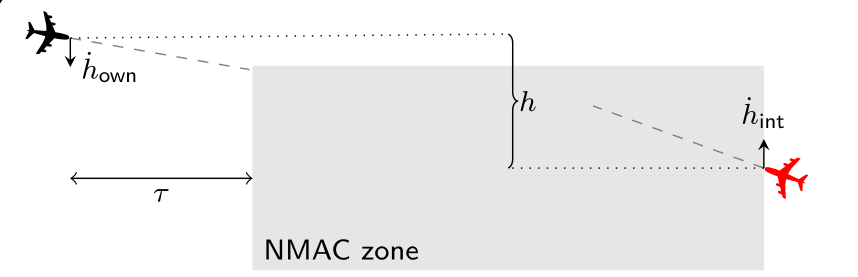
\includegraphics[width=7cm]{images/acas.png}};
    \end{tikzpicture}
    \end{figure}

%\blfootnote{M. Akintunde, E. Botoeva, {\bf P. Kouvaros}, A. Lomsucio. {{\em  Verifying Strategic Abilities of Neural-symbolic Multi-agent Systems}}. KR20}

\end{frame}

%%%%%%%%%%%%%%%%%%%%%%%%%%%%%%%%%%%%%%%%%%%%%%%

\begin{frame}{Two-agent Aircraft Collision Avoidance}

  \begin{itemize}\itemsep 1em
  \item %We verify instances of VCAS2 against the specifications:
    $ \varphi = \egamma[ag]{k} (\text{safe})$ \quad ({\it the ownship has a strategy to enter a safe
    configuration after $k$ time steps})    
  \item  $I = [h_I-2, h_I+2] \times \{-5.0\} \times \{5.0\} \times \{25\} \times \{\text{COC}\} \times \{\text{COC}\}$
  \end{itemize}

    \begin{figure}
    \begin{tikzpicture}
    \node [fig] (1) {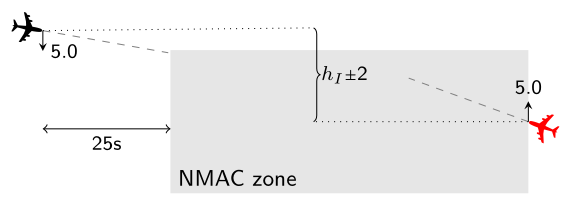
\includegraphics[width=6cm]{images/acas2.png}};
    \node [fig, below of = 1, yshift=-4em] (1) {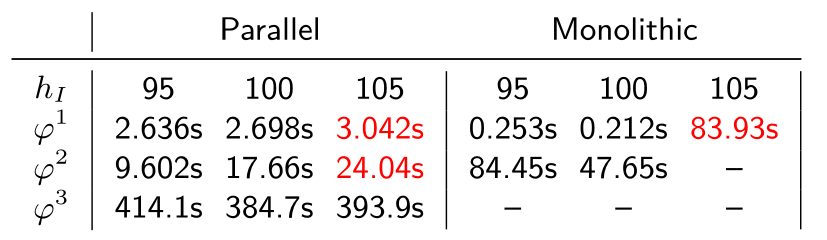
\includegraphics[width=7cm]{images/acas_exps.png}};
    \end{tikzpicture}
    \end{figure}
 
%\blfootnote{M. Akintunde, E. Botoeva, {\bf P. Kouvaros}, A. Lomsucio. {{\em  Verifying Strategic Abilities of Neural-symbolic Multi-agent Systems}}. KR20}

\end{frame}



%%%%%%%%%%%%%%%%%%%%%%%%%%%%%%%%%%%%%%%%%%%%%%%%%%%%%%%%%%%


\begin{frame}{Conclusions and Future Work}

\begin{itemize} \itemsep 2em

    \item Significant progress in the formal verification for AI 

    \item Scalability remains an issue

    \item Focus mostly on a limited repertoire of specifications 

    \item Robust training and neuro-symbolic learning

    \item Verification for unbounded systems of neuro-symbolic agents
\end{itemize}

%\end{itemize}

%\begin{itemize} \itemsep 1.5em

    %\item {\bf Scalable neural network verification} (optimised symbolic bound
        %propagation, GPU parallelisation, group dependencies, custom
        %branch-and-bound, SDP relaxations)

    %\item Neural network {\bf robustification} and  {\bf neuro-symbolic learning}

    %\begin{itemize} \itemsep 1em
        %\item[\textcolor{black}{-}] incorporation of the output of the verification step into the loss function towards {\em maximally} satisfying {\em soft constraints}

        %\item[\textcolor{black}{-}]  synthesis of neural network architectures towards satisfying {\em hard constraints}
    %\end{itemize}

    %\item {\bf Neuro-symbolic MAS} (abstractions, compositional reasoning)

    %\item {\bf Applications} (autonomous driving, aviation, medical imaging, finance, natural language processing)

%\end{itemize}

\end{frame}


%%%%%%%%%%%%%%%%%%%%%%%%%%%%%%%%%%%%%%%%%%%%%%%%

\end{document}
